\chapter{Experimantal Setup}
\label{ch:ExSetup}

Chapter \ref{ch:PotenHWSetup} discussed the possible options to implement a MIMO setup. The first option (Section \ref{sec:USRP}) was not viable due to technical limitations as it is described in Appendix \ref{sec:USRPSync}.

The second option (Section \ref{sec:MIMOAFW}) was financially unfeasible as the additional hardware for the modular MIMO set was to cost over €100.000. The only viable option was to use the LTE AFW with a MIMO Extension, although limited to a 2x2 MIMO system, was sufficient in this case.

\section{LTE Application Framework MIMO Extension}\label{sec:LTEAFWMIMOExt}

LTE AFW is a SISO LTE Release 10 implementation, where as LTE AFW 2x2 MIMO Extension was developed internally by NI as a plugin to the SISO framework to demonstrate a proof of concept for their MIMO Application Framework product. The main goal of LTE 2x2 MIMO Extension was to demonstrate a functioning 2x2 MIMO System. It is implemented for \textbf{DL only}. The software is not readily available for customers to purchase, but it was given to MSV as a workaround for the MIMO implementation.

For the implementation of the LTE AFW MIMO Extension as outlined in Chapter \ref{sec:LTEAFW} the equipment required is minimal. A set of 2 USRPs, one acting as a UE (Receiver) and the other acting as a Base Station (eNodeB) completes the transceiver chain and the Host PC does the graphing, data visualisation, user data communications and device setup. Figure \ref{fig:LTEAFWHWSetup} illustrates the simple HW connections required to make the device communicate with the host. For details on the part descriptions refer to Section \ref{ssec:LTEAFWHW}.

\begin{figure}[!htb]
    \centering
    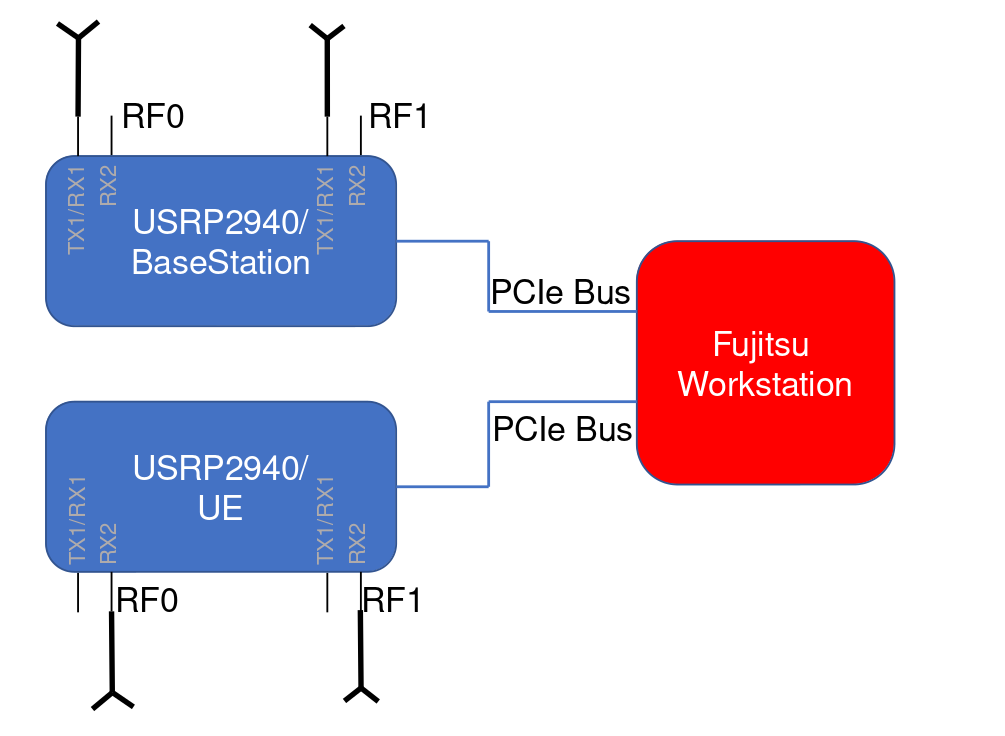
\includegraphics[width=11cm]{images/MIMOSetUpArrangement.png}
    \caption{Overview of the LTE 2x2 MIMOHW Connections}
    \label{fig:LTEAFWHWSetup}
\end{figure}


\subsection{LTE AFW MIMO Extension Architecture}\label{ssec:LTEAFWArch}

\begin{figure}[!htb]
    \centering
    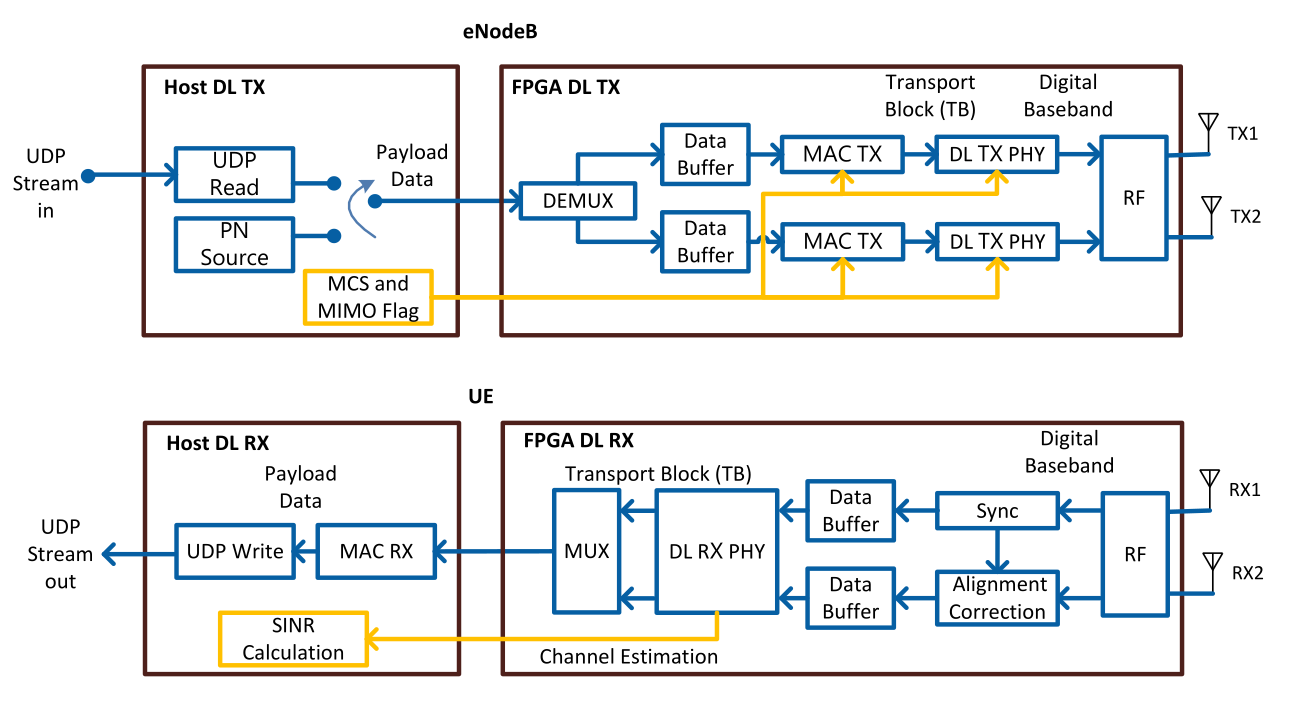
\includegraphics[width=\linewidth]{images/LTEAFW2x2ExtBlockDiagram.png}
    \caption{Overview of a 2 device Tx-Rx setup as intended in the final implementation}
    \label{fig:LTEAFW2DeviceOverview}
\end{figure}

Figure %s \ref{fig:LTEAFWExtArch} and 
\ref{fig:LTEAFW2DeviceOverview} shows the block diagram of the system in the DL, eNodeB and UE operation modes. Data streams that require high data rates for data transfer between host and FPGA are implemented as DMA FIFOs. These streams include the payload and UL data from host to FPGA and the received PDSCH/PUSCH transport blocks from FPGA to host. In-phase/quadrature (I/Q) samples for constellation and spectrum display as well as the channel estimation (\textbf{ONLY} \textit{h11} and \textit{h22}) values are also transferred from FPGA to host using DMA FIFOs. Further status information is transferred to the host by reading the indicator values \cite{LTEAFWManual}. As it can be seen both RX and TX components are implemented in the Host Software as well as in the FPGA Hardware. Hence the same application can be used as an \textit{eNodeB} as well as \textit{UE}. The \textit{eNodeB} mode uses the DL TX processing units and \textit{UE} uses the DL RX processing units which are explained in Section \ref{ssec:LTEAFWFPGA}. The following lists the various processing blocks in the application and a brief description of the corresponding tasks of each of the modules.

\begin{itemize}
    \item \textbf{UDP read} -
        Reads data, provided by an external application, from a UDP socket. The data is used as payload data in the transport block (TB). This data is then encoded and modulated as an LTE DL signal by the downlink transmitter (DL TX PHY).
    \item \textbf{UDP write} -
        Writes the payload data, which was received and decoded from the LTE DL signal by the downlink receiver (DL RX PHY), to a UDP socket. The data can then be read by an external application.
    \item \textbf{MCS and MIMO Flag} -
        Creates a cluster including the required information for the downlink control information (DCI) message such as the modulation and coding scheme (MCS) and the MIMO flag. The MIMO flag is a control that is used to activate MIMO or SISO in the eNodeB.
    \item \textbf{DEMUX} -
        A demultiplexer is used to split the data stream to Data Stream 1 and Data Stream 2 if the transmitter is configured to use both RF chains for TX. 
    \item \textbf{Data Buffer} -
        Two buffers are used to store data coming from the Payload H2T FIFO into two local FIFOs for TX chain 1 and TX chain 2. In the RX mode, two buffers are used to store the received data coming from the synchronization module to synchronize the signal processing in RX chain1 and RX chain 2.
    \item \textbf{MAC TX} -
        A simple MAC implementation that adds a header to the TB containing the number of payload bytes. The header is followed by the payload bytes, and the remaining bits of the TB are filled with padding bits.
    \item \textbf{DL TX PHY} -
        Physical layer (PHY) of the downlink (DL) transmitter (TX). Encodes the physical channels and creates the LTE downlink signal as digital baseband I/Q data. This code includes encoding of the control channel (PDCCH), encoding of the data channel (PDSCH), resource mapping, and orthogonal frequency-division multiplexing (OFDM) modulation. The white paper Labview communications LTE Application Framework 19.5\cite{LTEAFWManual} has the details of the implementation of the TX Bit Processing and IQ Signal Processing.
    \item \textbf{Sync} -
        The primary synchronization sequence (PSS) is used for synchronization. The synchronization is done using the received signal on RF0/RX2. The synchronization results such as frame alignment and frequency offsets estimation (integral and fractional) are used to adjust the received signals on both ports RF0/RX2 and RF1/RX2.
    \item \textbf{DL RX PHY} -
        Physical layer (PHY) of the downlink (DL) receiver (RX). Demodulates the LTE downlink signal and decodes the physical channels, OFDM demodulation, resource demapping, MIMO channel estimation and MIMO equalization, decoding of the control channel (PDCCH), and decoding of the data channel (shared channel, PDSCH). For MIMO equalization, three algorithms have been implemented namely: simple algorithm, minimum mean squared error (MMSE), and zero-forcing (ZF). The simple algorithm means that the inverse of the estimated channel parameters is used directly in the equalizer. There is also an option of disabling the equalization using a switch to get raw data.
    \item \textbf{MUX} -
        A multiplexer is used to combine the received data from both RX chains to be transmitted to the host.
    \item \textbf{MAC RX} -
        Disassembles the TB and extracts the payload bytes.
    \item \textbf{SINR calculation} -
        Calculates the signal-to-interference-noise-ratio (SINR) based on the channel estimation that was used for PDSCH decoding. Channel estimation is either based on cell-specific reference signals (CRS), or on UE-specific reference signals (UERS).
    \item \textbf{RF} -
        In the transmit path, it performs digital up conversion (DUC), RF impairments correction, and writes the transmit data to the RF. In the receive path, it reads the received data from the RF, performs digital down conversion (DDC) and performs RF impairments correction.
\end{itemize}

%\begin{figure}[H]
%    \centering
%    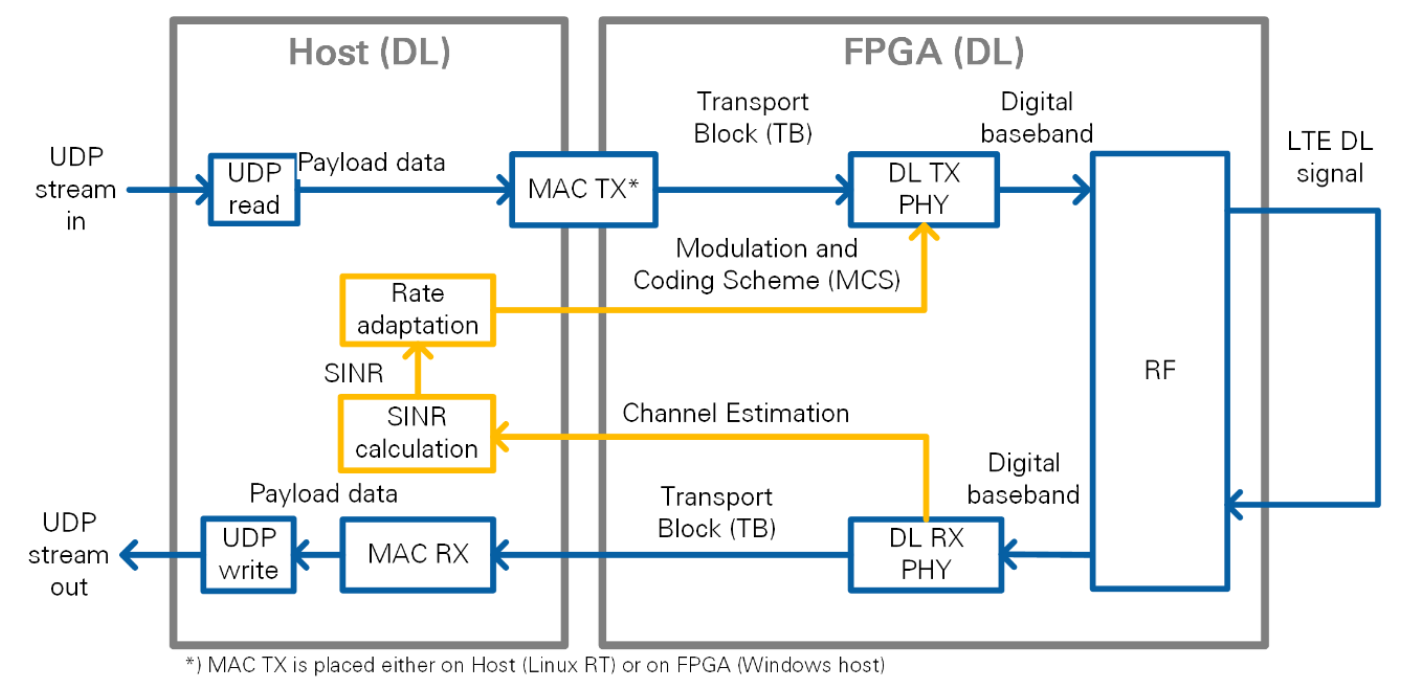
\includegraphics[width=11.5cm]{images/LTEAFWExtArch.png}
%    \caption{Overview of the LTE 2x2 MIMO Architecture and the HW/SW design split}
%    \label{fig:LTEAFWExtArch}
%\end{figure}

\subsection{LTE AFW Host Software}\label{ssec:LTEAFWHostSW}
The LTE AFW 2x2 MIMO application uses a UDP stream to transfer data between the host and the device or vice versa. Figure \ref{fig:UDPDataTransfer} shows the end to end data flow starting from the host, going through the data FIFOs set up in the FPGAs and back to the host again where the received data is displayed.

\begin{figure}[H]
    \centering
    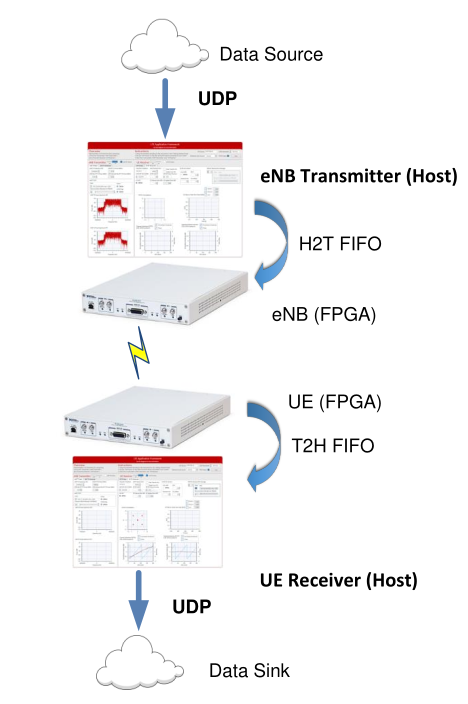
\includegraphics[width=8cm]{images/UDPDataTransfer.png}
    \caption{UDP Host-Device Data transfer}
    \label{fig:UDPDataTransfer}
\end{figure}

\subsubsection{Host Software Modifications}\label{ssec:LTEAFWHostSWMods}
The host software was heavily modified for the following reasons

\begin{itemize}
    \item The version of the software given to MSV by NI was intended for an older version \textit{LabVIEW Communication System Design Suite 2.0} which was only supported for all OS releases until Windows 8.1/7 64-bit.

    \item The FPGA source was not issued to MSV instead a pre compiled FPGA bit file was delivered, but this corresponded to the \textbf{old} version namely \textit{Labview Communications System Design Suite 2.0}.

    \item The project was not forwards compatible with the latest version of the Labview Communications System Design Suite.
\end{itemize}

As a result of the above mentioned point and to guarentee future compatibility, the project had to be ported to the latest version of \textit{LabVIEW Communication System Design Suite 4.0}, which was renamed as \textit{Labview NXG 4.0}. Missing dependencies had to be manually included and many driver related functionalities had to be modified as the newer version had a different driver implementation compared to the older version.

\subsubsection{DL Receiver}\label{ssec:LTEAFWRXOptions}

The DL Receiver implements the end to end receiver chain from receiving the raw data from the RF Frontend to the OFDM processing, demodulation and LTE processing steps. Most of the complex resource intensive data processing is done onboard the FPGA as mentioned in Section \ref{ssec:LTEAFWFPGA}. Certain parameters of the receiver can be manually configured according to user specifications. The chosen settings for this experiment are listed in Table \ref{tab:RXUSRPParam}.

\begin{table}[H]
    \begin{center}
        \begin{tabular}{|l|l|}
            \hline
            \textbf{Parameter}                                                          & \textbf{Value} \\ \hline
            Center Frequency                                                            & 1.2\si{\giga\hertz}         \\ \hline
            Transmit IP Address	                                                        &
127.0.0.1      \\ \hline
            UDP Receive Port                                                            & 60000          \\ \hline
            \begin{tabular}[c]{@{}l@{}}Receiver RX Antenna \\ Port On USRP\end{tabular} & RX2/RF1        \\ \hline
                Cell ID                                                                     & 0              \\ \hline
                LTE Duplexing Mode                                                          & FDD            \\ \hline
                Manual Receiver Gain                                                        & 20\si{\dB}           \\ \hline
        \end{tabular}
        \caption{Receiver USRP Parameters Setup}
        \label{tab:RXUSRPParam}
    \end{center}
\end{table}

The DL RX (UE) mode screens are shown in Figures \ref{fig:DLRXScreen} and \ref{fig:DLRXAdvScreen}.

\begin{figure}[H]
    \centering
    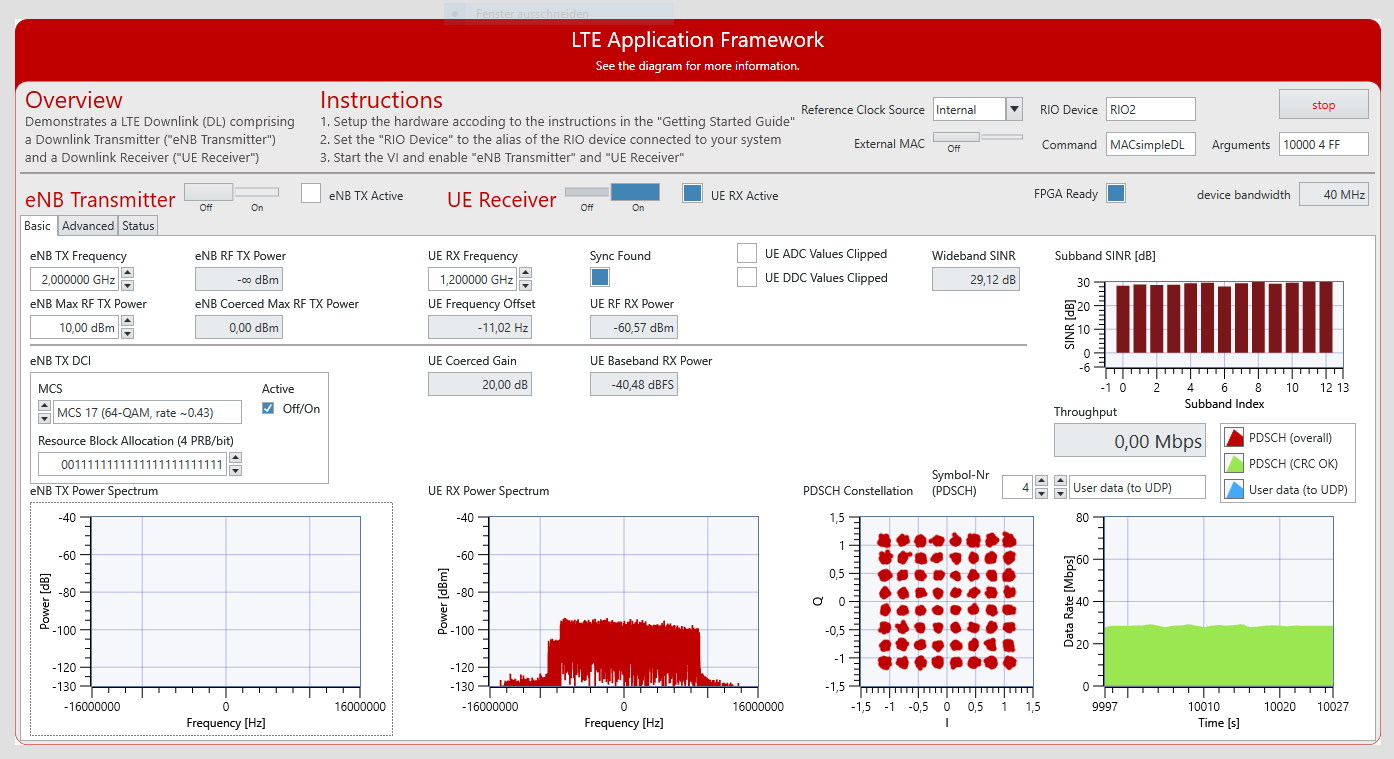
\includegraphics[width=\linewidth]{images/SISORXEdited.png}
    \caption{A Screencapture of the DL RX(UE) side application window}
    \label{fig:DLRXScreen}
\end{figure}

\begin{figure}[H]
    \centering
    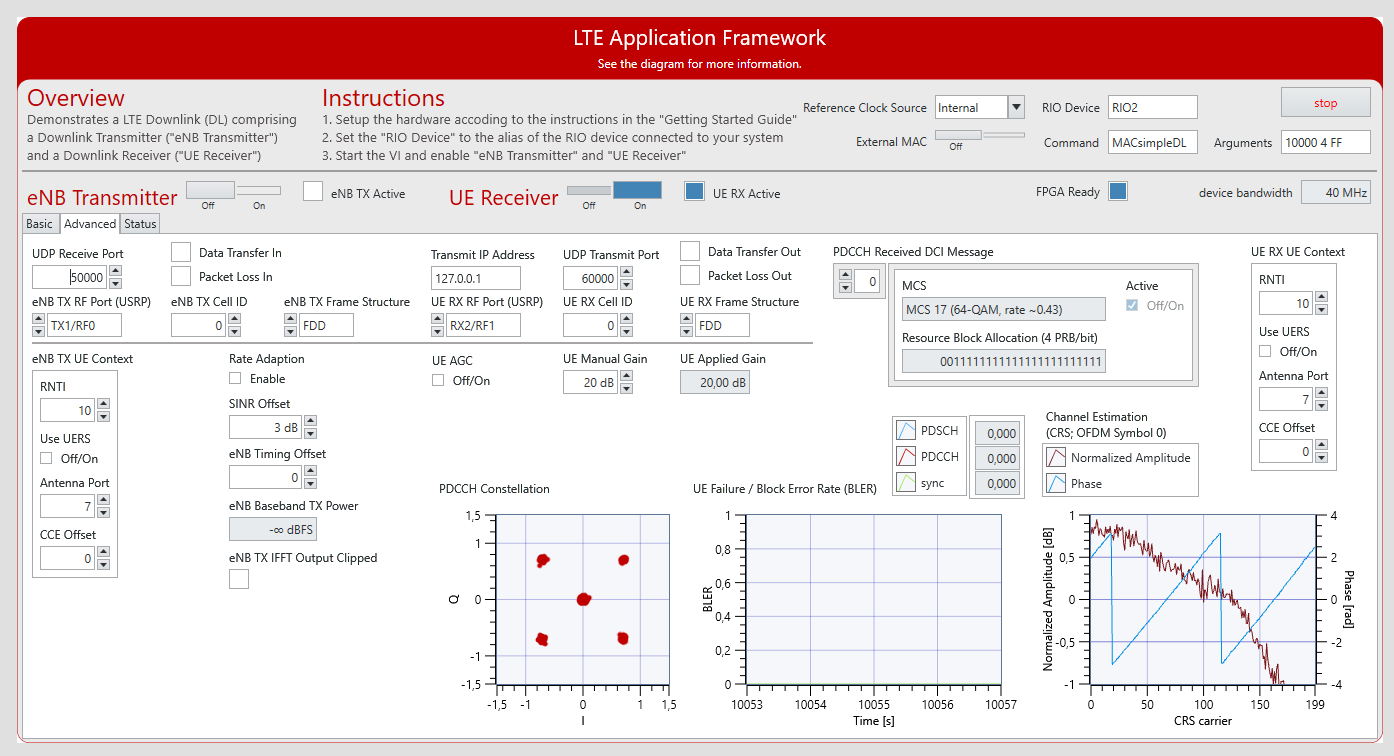
\includegraphics[width=\linewidth]{images/SISORXADVEdited.png}
    \caption{A Screencapture of the DL RX(UE) Advanced Options in the application window}
    \label{fig:DLRXAdvScreen}
\end{figure}

Table \ref{tab:RXUSRPParamDesc} describes the various graphs and indicators shown on the RX screen of the application.

\begin{landscape}
    % Please add the following required packages to your document preamble:
    % \usepackage[normalem]{ulem}
    % \useunder{\uline}{\ul}{}
    \begin{table}[]
        \begin{tabular}{|l|p{14cm}|}
            \hline
            \textbf{Indicator}         & \textbf{Description}                                                                                                                                                                                                                                                                  \\ \hline
            MIMO flag                  & Activates the eNodeB to run in MIMO setup. The MIMO flag is included in the DCI message to be deciphered at the RX part of UE.                                                                                                                                                        \\ \hline
            Equalizer Type             & Configures the algorithm that is used for equalization. The enumeration contains the following values: MMSE, ZF, and Simple.                                                                                                                                                          \\ \hline
            Sigma                      & Selects the scaling factor that is used in the MMSE channel equalizer.                                                                                                                                                                                                                \\ \hline
            MIMO Selector AP0          & Determines the PDSCH Constellation of AP0 that has been derived from SISO equalizer or MIMO equalizer.                                                                                                                                                                                \\ \hline
            eNB TX Power Spectrum AP0  & Shows the power spectrum of the DL TX baseband signal transferred to the RF0/TX1.                                                                                                                                                                                                     \\ \hline
            eNB TX Power Spectrum AP1  & Shows the power spectrum of the DL TX baseband signal transferred to the RF1/TX1.                                                                                                                                                                                                     \\ \hline
            UE RX Power spectrum AP0   & Shows the power spectrum of the DL RX baseband signal received from RF0/RX2.  If synchronization is successful based on the received signal from RX1 (RF0/RX2), frame timing and frequency offset correction are applied on the received signals from both ports RF0/RX2 and RF1/RX2. \\ \hline
            UE RX Power spectrum AP1   & Shows the power spectrum of the DL RX baseband signal received from RF1/RX2.                                                                                                                                                                                                          \\ \hline
            PDSCH Constellation of AP0 & Constellation of RX IQ samples of AP0 allocated for PDSCH transmission after SISO or MIMO equalization. Only samples for the configured OFDM Symbol-Nr (PDSCH) are displayed.                                                                                                         \\ \hline
            PDSCH Constellation of AP1 & Constellation of RX IQ samples of AP1 allocated for PDSCH transmission after MIMO equalization. Only samples for the configured OFDM Symbol-Nr (PDSCH) are displayed.                                                                                                                 \\ \hline
            Channel Estimation of AP0  & Graphical representation of the normalized channel amplitude and phase estimated based on the cell specific reference signals of AP0                                                                                                                                                  \\ \hline
            Channel Estimation of AP1  & Graphical representation of the normalized channel amplitude and phase estimated on the cell specific reference signals of AP1.                                                                                                                                                       \\ \hline
        \end{tabular}
        \caption{Receiver USRP indicators description}
        \label{tab:RXUSRPParamDesc}
    \end{table}
\end{landscape}

\subsubsection{DL Transmitter}\label{ssec:LTEAFWTXOptions}

\subsection{LTE AFW FPGA}\label{ssec:LTEAFWFPGA}
LTE has demanding and resource intensive processing requirements and in the application framework, the processing blocks for the DL and UL TX and RX are implemented directly on the FPGA. They exchange the baseband data with the RF interface using target-scoped FIFOs. The processing on the FPGA has advantages because it provides lower latency and therefore enables real-time physical layer processing. The following section describe the steps involved in the DL TX and DL RX processing done on the FPGA.

\subsubsection{DL TX IQ Processing}\label{sssec:DLTXIQProc}

\begin{figure}[!htb]
    \centering
    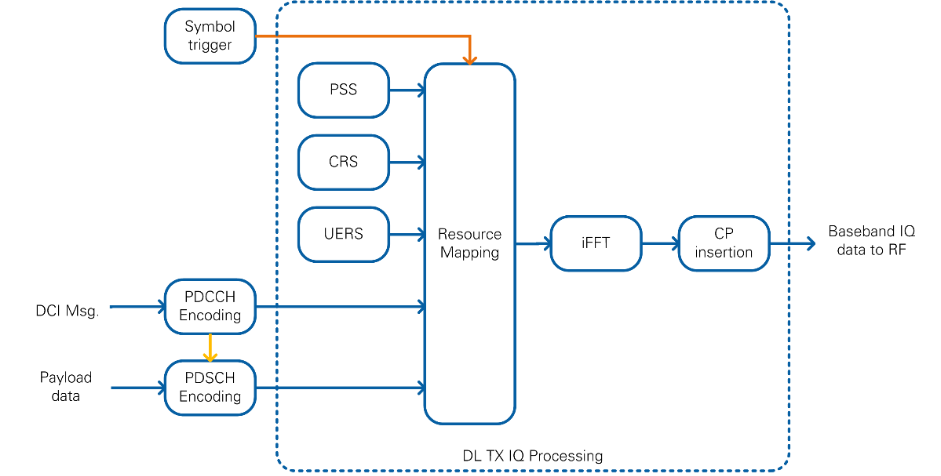
\includegraphics[width=\linewidth]{images/DLFPGATXImpl.png}
    \caption{Simplified implementation of the DL TX processing block of the FPGA}
    \label{fig:LTEAFWFPGADLTXProc}
\end{figure}

\subsubsection{DL RX IQ Processing}\label{sssec:DLRXIQProc}

This module reads the radio-frame aligned signal in time domain and outputs the channel-equalized subcarriers that are associated to the physical channels. As shown in Figure \ref{fig:LTEAFWFPGADLRXProc}, it includes the following functional blocks

\begin{figure}[!htb]
    \centering
    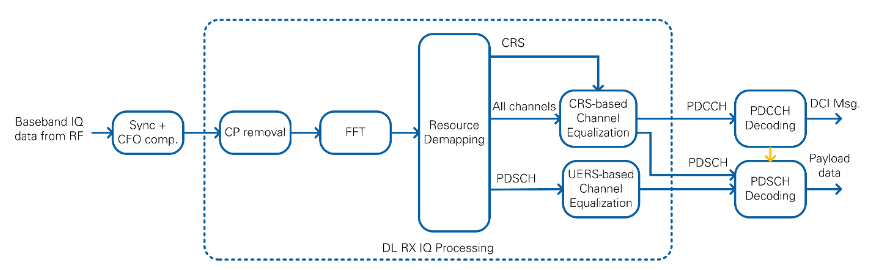
\includegraphics[width=\linewidth]{images/DLFPGARXImpl.png}
    \caption{Simplified implementation of the DL RX processing block of the FPGA}
    \label{fig:LTEAFWFPGADLRXProc}
\end{figure}

\begin{itemize}
    \item \textbf{Radio Frame Synchronization} -
        Synchronization is vital for the time alignment of the Frames as OFDM is extreamly time sensitive. CFO (Carrier Frequency Offset) correction is important to correct for any error/inaccuracies in the local oscilators. This could inadvertently move the frequency grid up or down based on the offset. Synchronization and CFO compensation are achieved by continuous measurement of both an autocorrelation and a cross correlation. LTE signals contain a PSS, which is detected by two finite impulse response (FIR) filters (real and imaginary part) that calculate the cross correlation. This operation is executed on a reduced sample rate of 1.92 MS/s, which is the result of a decimation by 16. For each radio frame, the cross correlation peak is detected. To avoid misdetection, a validation unit checks that the peak amplitude is eight times higher than the average energy of the cross correlation. Additionally, three consecutive peaks are required, and the peak position may not drift more than five samples.
    \item \textbf{CP removal} -
        An internal FIFO is used to decouple the incoming samples from the rest of the processing chain. The throttle control module waits until enough samples for one complete OFDM symbol (FFT size + CP) are available before it passes them as a consecutive stream to the next modules. The CP removal removes the valid flag from the samples belonging to the cyclic prefix. The 2,048 remaining samples are sent to a Xilinx FFT. For a full 20 \si{\mega\hertz} BW LTE system the number of samples in a subframe is 2048 plus the CP samples that are added during the TX process. Once the CP is removed the remaining 2048 Samples are forwarded onto the FFT Conversion module.
    \item \textbf{FFT Conversion} -
        The output of the FFT are 2048 the subcarriers in frequency domain.
    \item \textbf{Resource demapping} -
        The resource demapper selects the 1200 allocated subcarriers by removing the surrounding whitespace and the DC carrier in the center. Then it generates the timing information for each sample and the resource grid by marking each sample for its corresponding channel by using a Boolean cluster. The resource mapping is based on a fixed frame structure configuration described in the LTE specifications. All subsequent modules use this Boolean cluster with elements for each LTE channel to determine if this sample is relevant.
    \item \textbf{CRS based channel estimation and equalization} -
        The FFT output data is fed into two separate channel estimation blocks running in parallel. The first channel estimation is based on the CRS. The channel estimate values are calculated by conjugate complex multiplications. A linear interpolation is applied in frequency domain between adjacent reference symbols. On the edges of the symbol, the nearest estimated value is replicated (zero order hold). OFDM symbols not containing CRS sequences rely on the last channel estimation (zero order hold in time) as shown in Figure \ref{fig:ChEstInterpolation}
    \item \textbf{UERS based channel estimation and equalization} -
        This signalling scheme is available for use but not actively used in this thesis.
\end{itemize}

\begin{figure}%
    \centering
    \subfloat[Channel Estimation Interpolation over Frequency]{{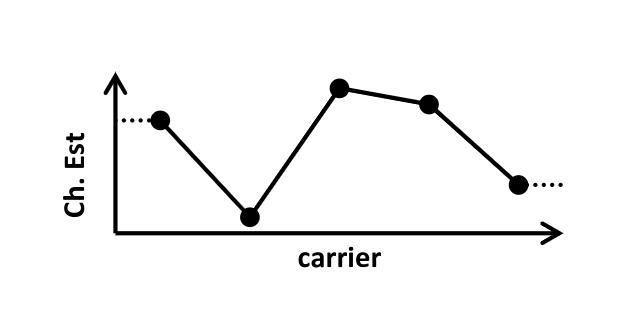
\includegraphics[width=5cm]{images/ChEstInterpolation.png} }}%
    \qquad
    \subfloat[Channel Estimation Zero order hold over time]{{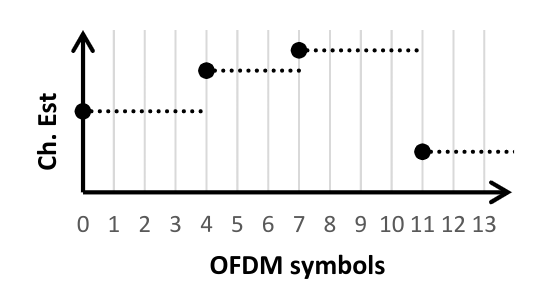
\includegraphics[width=5cm]{images/ChEstZOH.png} }}%
    \caption{Illustration of channel estimation interpolation over time and frequency}%
    \label{fig:ChEstInterpolation}%
\end{figure}

\section{Application Example}\label{sec:AppEx}
\begin{table}[H]
    \begin{center}
        \begin{tabular}{|c|c|}
            \hline
            \textbf{Coefficient Index} & \textbf{Coefficient Values} \\ \hline
            0                          & 0                           \\ \hline
            1                          & -0.061235467                \\ \hline
            2                          & 0                           \\ \hline
            3                          & 0.306177333                 \\ \hline
            4                          & 0.510116268                 \\ \hline
            5                          & 0.306177333                 \\ \hline
            6                          & 0                           \\ \hline
            7                          & -0.061235467                \\ \hline
            8                          & 0                           \\ \hline
        \end{tabular}
    \end{center}
\end{table}

